%%
% The BIThesis Template for experiment report
%
% Copyright 2020-2021 Silvester Wang, BITNP
%
% This work may be distributed and/or modified under the
% conditions of the LaTeX Project Public License, either version 1.3
% of this license or (at your option) any later version.
% The latest version of this license is in
%   http://www.latex-project.org/lppl.txt
% and version 1.3 or later is part of all distributions of LaTeX
% version 2005/12/01 or later.
%
% This work has the LPPL maintenance status `maintained'.
%
% The Current Maintainer of this work is Feng Kaiyu.
%
% Compile with: xelatex -> biber -> xelatex -> xelatex

\documentclass[lab-report]{bitart}


% 将你的相关信息替换如下示例
\newcommand{\reportName}{通信课程实验报告}
\newcommand{\deptName}{计算机学院}
\newcommand{\majorName}{计算机科学与技术}
\newcommand{\className}{07xxxxxx}
\newcommand{\yourName}{惠计算}
\newcommand{\teacherName}{张哈希}
% \newcommand{\coverDate}{2022年5月9日} % 注释此行以使用自定义日期

\addbibresource{misc/refs.bib}

\begin{document}

\section{实验目的}
\begin{enumerate}
  \item 验证抽样原理
  \item 观察了解 PAM 信号形成过程
  \item 了解混沌效应形成原因
\end{enumerate}

\section{实验仪器}
\begin{enumerate}
  \item ZH7001 通信原理综合实验系统
  \item 20MHz 双踪示波器
  \item 函数信号发生器
\end{enumerate}

\section{实验原理}
利用抽样脉冲把一个连续信号变为离散时间样值的过程称为抽样,抽样后的信号称为脉冲调幅(PAM)信号。抽样定理指出,一个频带受限的信号 $m(t)$,如果他的最高频率为 $f_h$,那么可以唯一的由频率大于或等于 $2f_h$ 的样值序列所决定,即可以由抽样序列无失真地还原原始信号,抽样序列保留原始信号的全部信息。

\section{实验过程}
\subsection{近似理想抽样脉冲序列测量}
函数信号发生器产生正弦信号,频率为 1 KHz,输出电平为 1Vp-p。

波形图如下图\ref{波形图}。

\begin{figure}[H]
  \centering
  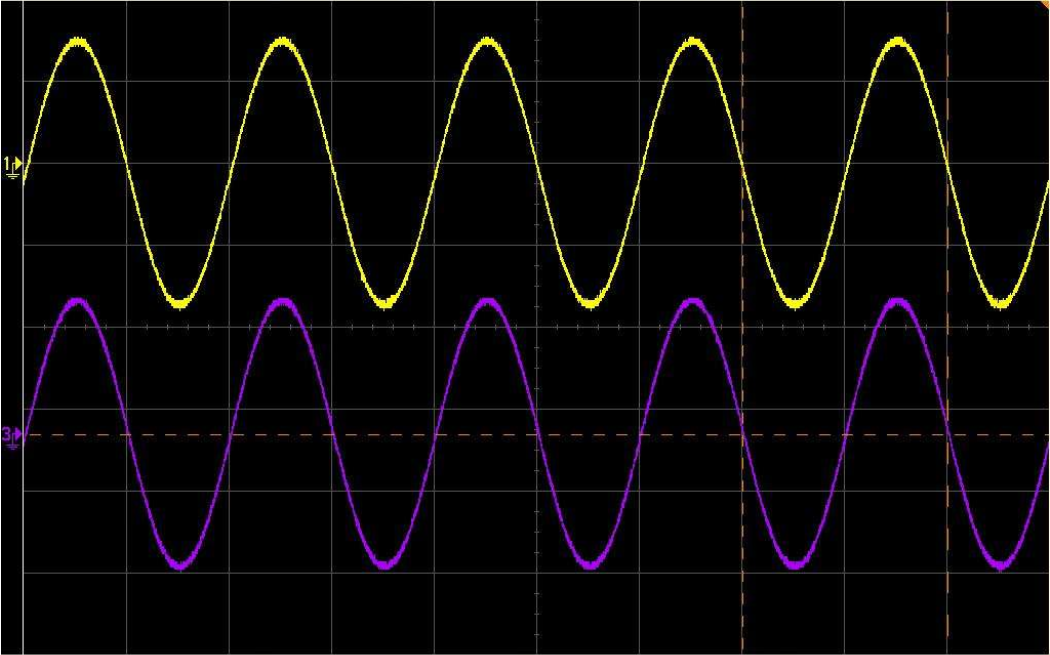
\includegraphics[width=0.63\textwidth]{assets/p1.jpg}
  \caption{波形图}
  \label{波形图}
\end{figure}

\subsection{理想抽样信号重建观察}
理想抽样信号

\section{实验总结}
通过这次实验,我从中知道了抽样原理。

\printbibliography[heading=bibliography,title=参考文献]

\end{document}
